\section{51 - MAT - FA 1.4, AN 2.1, AN 3.3, AN 4.2 - Lorenz-Kurve - Matura 2014/15 1. Nebentermin}

\begin{langesbeispiel} \item[0] %PUNKTE DES BEISPIELS
				
	Der US-amerikanische Statistiker Max Otto Lorenz entwickelte im Jahr 1905 zur Veranschaulichung von Einkommensverteilungen die Lorenz-Kurve. Für die Darstellung der Lorenz-Kurve ordnet man die Haushalte eines Staates nach der Höhe ihres Einkommens.  Die Lorenz-Kurve gibt für jeden Prozentsatz der Haushalte an, wie viel Prozent des Volkseinkommens auf ihn entfallen. So steht jeder Punkt $P=(x|y)$ auf der Kurve für folgende Aussage: "`Die unteren $x\,\%$ aller Haushalte beziehen $y\,\%$ des Gesamteinkommens."' Die nachstehende Abbildung zeigt die Lorenz-Kurve von Österreich für das Jahr 2009. 
				
				\begin{center}
					\resizebox{0.7\linewidth}{!}{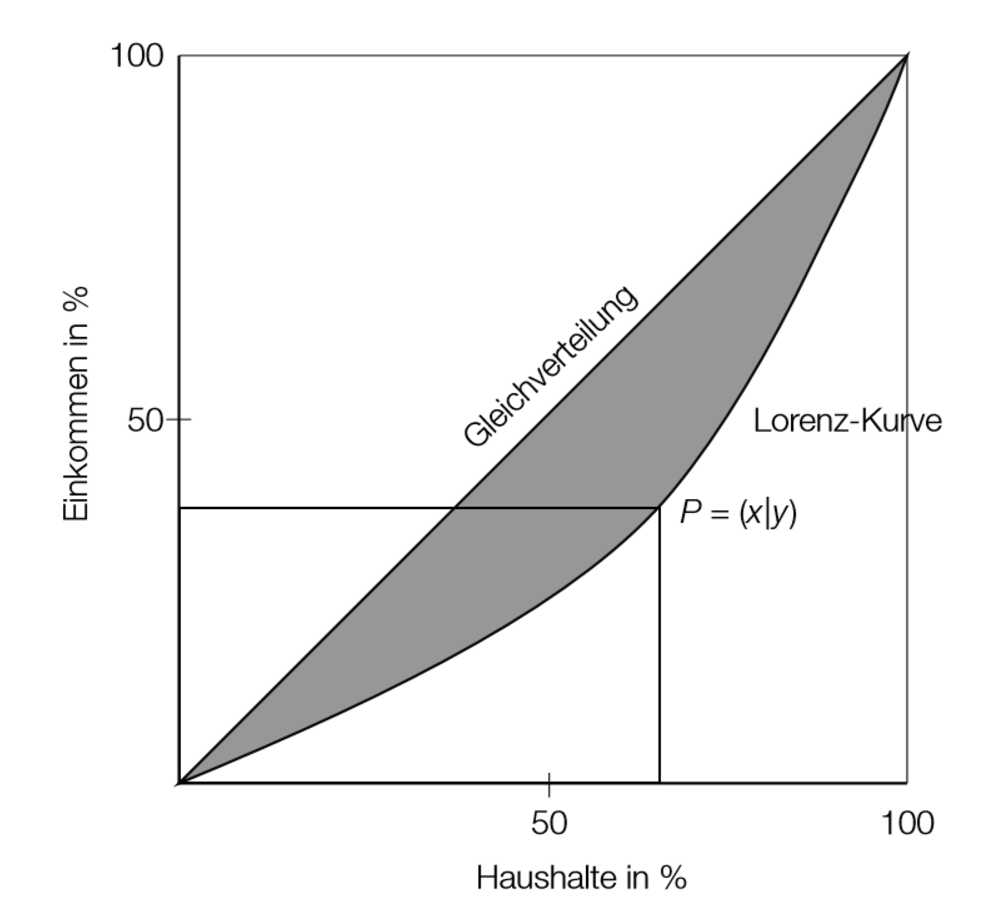
\includegraphics{../Bilder/Bild51-1.eps}}
				\end{center}
				\begin{singlespace}\begin{scriptsize} Quelle: http://diepresse.com/home/wirtschaft/economist/446997/Sozialbericht\_Einkommen-in-Oesterreich-ungleicher-verteilt [26.05.2015] (bearbeitet)\end{scriptsize}\end{singlespace}
				
				Nimm an, dass die Lorenz-Kurve eines Landes durch die Funktion $f$ mit
				$$f(x)=4\cdot 10^{-7}\cdot x^4+2\cdot 10^{-3}\cdot x²+4\cdot 10^{-1}\cdot x$$
				und die Gleichverteilungsgerade durch die Funktion $g$ mit
				$$g(x)=x$$
				modelliert werden können ($x$ in \%; $f(x)$ in \%; $g(x)$ in \%). Die nachstehende Abbildung zeigt die Graphen der Funktionen $f$ und $g$. Der charakteristische "`Bauch"' der Lorenz-Kurve unterhalb der Diagonalen ist ein Maß für die Ungleichverteilung der Einkommen. Er ist in der Abbildung schraffiert dargestellt.
				
				\begin{center}
					\resizebox{0.7\linewidth}{!}{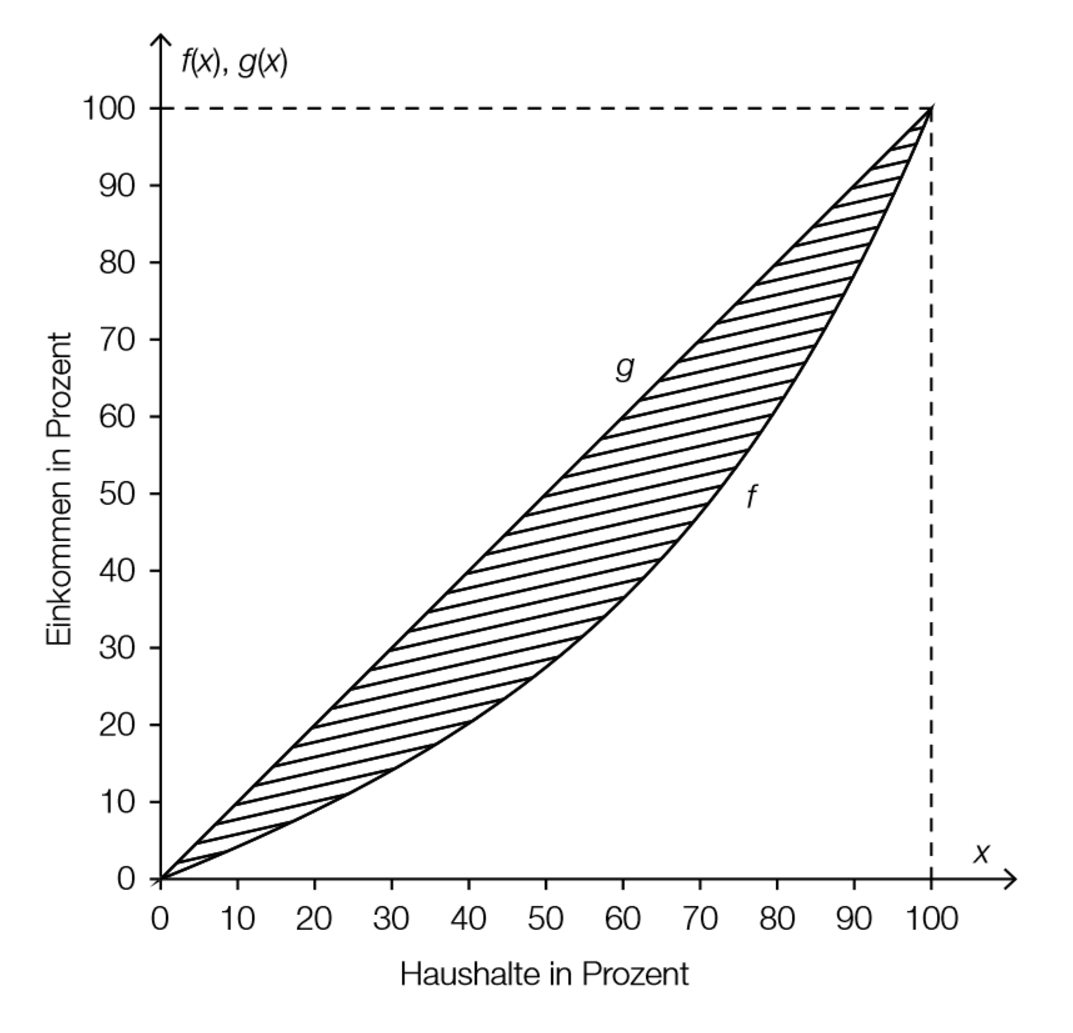
\includegraphics{../Bilder/Bild51-2.eps}}
				\end{center}

\subsection{Aufgabenstellung:}
\begin{enumerate}
	\item \fbox{A} Berechne, wie viel Prozent des Gesamteinkommens auf die reichsten $20\,\%$ der Haushalte des Landes entfallen!
	
	Zeige mithilfe der Differenzialrechnung, dass die Funktion $f$ im Intervall $[0;100]$ linksgekrümmt ist!
	
\item Der Gini-Koeffizient ist der Anteil der schraffierten Fläche an der Fläche zwischen der Gleichverteilungsgeraden und der $x$-Achse im Intervall $[0; 100]$.  

Berechne den Gini-Koeffizienten des Landes mit der Lorenz-Kurve $f$!\leer

 
 Gib den Gini-Koeffizienten für einen Staat an, in dem alle Haushalte gleich viel verdienen!
						\end{enumerate}\leer
				
\antwort{
\begin{enumerate}
	\item \subsection{Lösungserwartung:} 
	
	$100-f(80)=38,816$\leer
	
	Es entfallen ca. 38,8\,\% des Gesamteinkommens auf die reichsten 20\,\% der Haushalte.\leer
	
	$f(x)=4\cdot 10^{-7}\cdot x^4+2\cdot 10^{-3}\cdot x²+4\cdot 10^{-1}\cdot x$
	
	$f'(x)=1,6\cdot 10^{-6}\cdot x³+4\cdot 10^{-3}\cdot x+4\cdot 10^{-1}$
	
	$f''(x)=4,8\cdot 10^{-6}\cdot x²+4\cdot 10^{-3}$\leer
	
	Die Funktion $f$ ist linksgekrümmt, weil: $f''(x)=4,8\cdot 10^{-6}\cdot x²+4\cdot 10^{-3}>0$ für alle $x\in [0;100]$.
		
	\subsection{Lösungsschlüssel:}
	\begin{itemize}
		\item Ein Ausgleichspunkt für die richtige Lösung. Äquivalente Schreibweisen des Ergebnisses (als Bruch oder Dezimalzahl) sind ebenfalls als richtig zu werten.  
		
		Toleranzintervalle: $[38\,\%; 39\,\%]$ bzw. $[0,38; 0,39]$
		\item  Ein Punkt für eine (sinngemäß) korrekte Begründung.
	\end{itemize}
	
	\item \subsection{Lösungserwartung:}
			
		$A_1=\int^{100}_0{f(x)}$d$x=3\,466,\bar{6}$
		
		$A_2=\frac{100\cdot 100}{2}=5\,000$
		
		$\frac{A_2-A_1}{A_2}=\frac{1\,533,\bar{3}}{5\,000}=0,30\bar{6}\approx 0,31$
		
		Der Gini-Koeffizient für das Land mit der Lorenz-Kurve $f$ beträgt 0,31.\leer
		
		$\frac{0}{5\,000}=0$
		
		Der Wert des Gini-Koeffizienten für einen Staat, in dem alle Haushalte gleich viel verdienen beträgt 0.

	\subsection{Lösungsschlüssel:}
	
\begin{itemize}
	\item  Ein Punkt für die richtige Lösung.  
	
	Toleranzintervall: $[0,30; 0,31]$  
	
	Die Aufgabe ist auch dann als richtig gelöst zu werten, wenn bei korrektem Ansatz das Ergebnis aufgrund eines Rechenfehlers nicht richtig ist. 
	\item Ein Punkt für die richtige Lösung.
\end{itemize}

\end{enumerate}}
		\end{langesbeispiel}